\documentclass{standalone}
\usepackage{tikz}
\usepackage{animate}
\usepackage{amsmath}
\usepackage{ifthen}
\usetikzlibrary {matrix}
\usepackage{tikzlings}
\usepackage{tikzlings-penguins}

\begin{document}
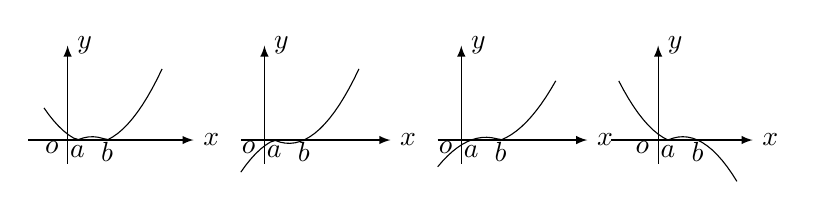
\begin{tikzpicture}[>=latex,domain=-0.3:1.2]
 \xdef\a{0.125} 
 \xdef\b{0.5}
 \xdef\scale{1.2}
 \xdef\ppos{-0.6}
  \begin{scope}
    \draw[->] (-0.5,0) -- (1.6,0) node[right] {$x$};
    \draw[->] (0,-0.3)--(0,1.2) node[right] {$y$};
    \node (a) at (\a,-0.15) {$a$};
    \node (b) at (\b,-0.15) {$b$};
    \node (o) at (-0.2,-0.1){ $o$};
    \draw plot (\x,{\scale*abs(\x-\a)*abs(\x-\b)});
  \end{scope}
  \begin{scope}[xshift=2.5cm]
    \draw[->] (-0.3,0) -- (1.6,0) node[right] {$x$};
    \draw[->] (0,-0.3)--(0,1.2) node[right] {$y$};
    \node (a) at (\a,-0.15) {$a$};
    \node (b) at (\b,-0.15) {$b$};
    \node (o) at (-0.2,-0.1){ $o$};
    \draw plot (\x,{\scale*abs(\x-\a)*(\x-\b)});
  \end{scope}
  \begin{scope}[xshift=5cm]
    \draw[->] (-0.3,0) -- (1.6,0) node[right] {$x$};
    \draw[->] (0,-0.3)--(0,1.2) node[right] {$y$};
    \node (a) at (\a,-0.15) {$a$};
    \node (b) at (\b,-0.15) {$b$};
    \node (o) at (-0.2,-0.1){ $o$};
    \draw plot (\x,{\scale(\x-\a)*abs(\x-\b)});
  \end{scope}
  \begin{scope}[xshift=7.5cm,domain=-0.5:1]
    \draw[->] (-0.6,0) -- (1.2,0) node[right] {$x$};
    \draw[->] (0,-0.3)--(0,1.2) node[right] {$y$};
    \node (a) at (\a,-0.15) {$a$};
    \node (b) at (\b,-0.15) {$b$};
    \node (o) at (-0.2,-0.1){ $o$};
    \draw plot (\x,{\scale*-1*abs(\x-\a)*(\x-\b)});
  \end{scope}
\end{tikzpicture}


\end{document}
